\begin{figure}
	\centering
	\begin{subfigure}{0.48\columnwidth}
		\centering
		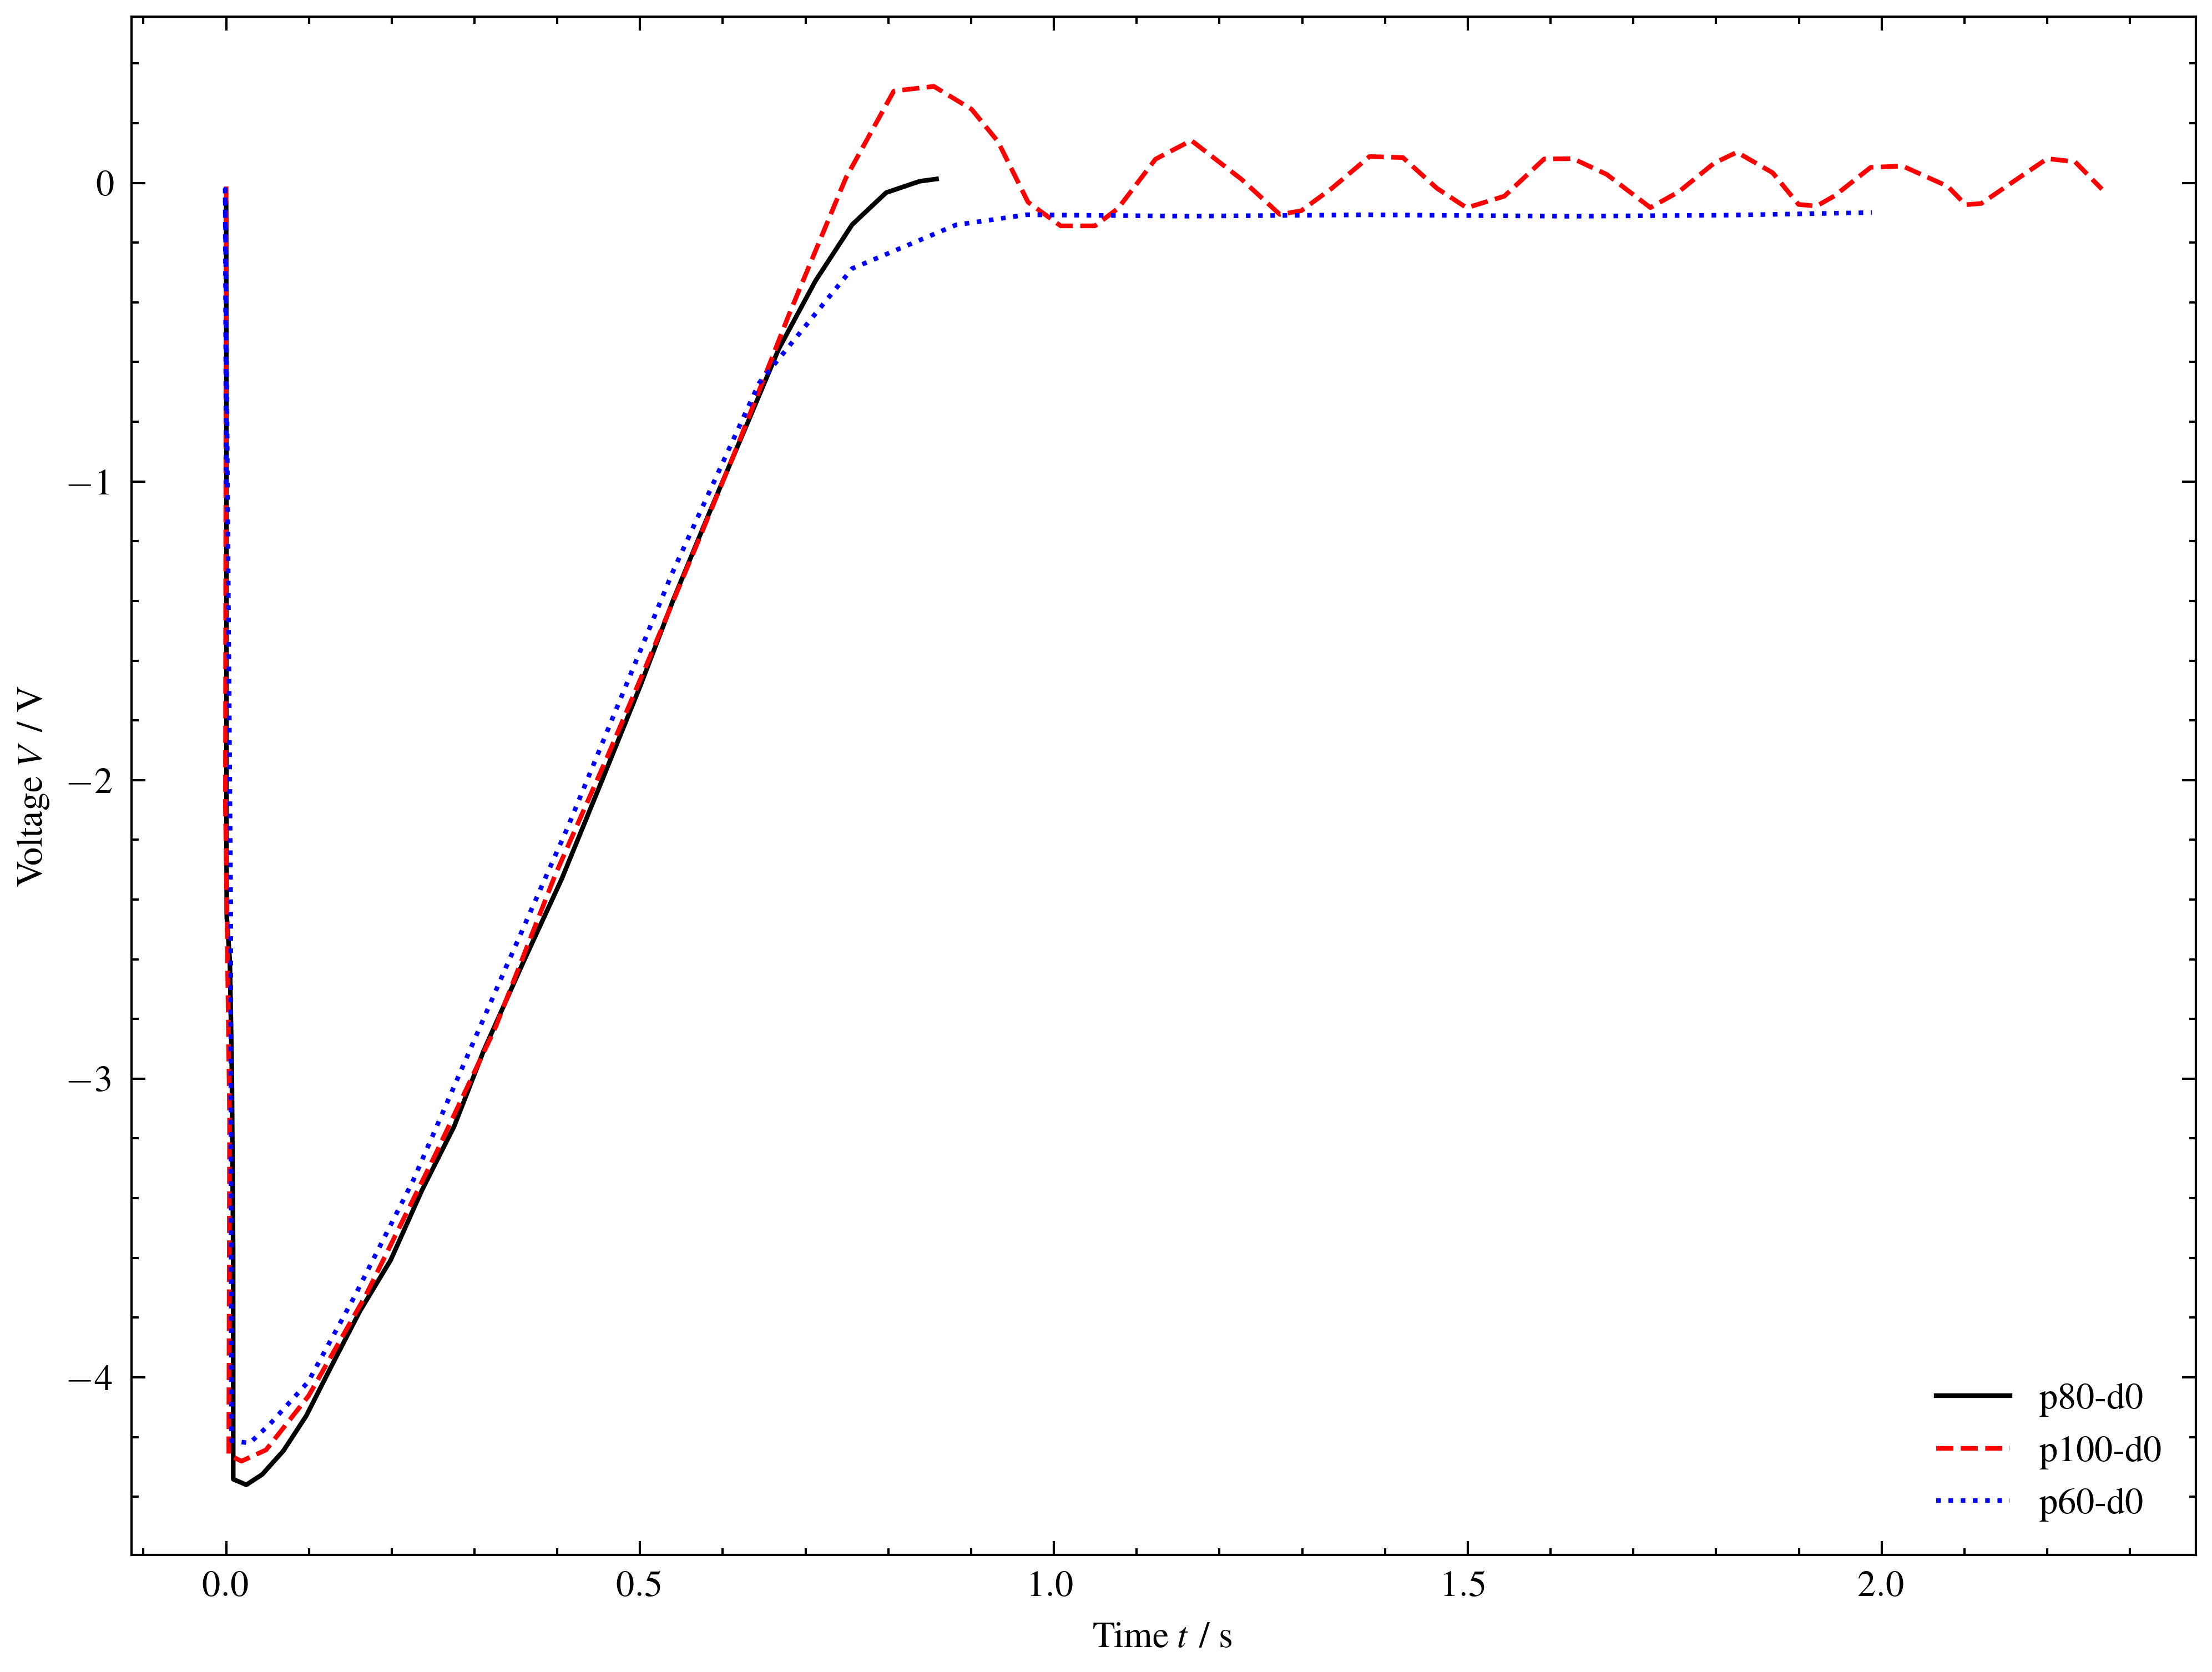
\includegraphics[width=0.8\linewidth]{src/figures/oscilloscope-grouped/d-0.png}
		\subcaption{$D = 0$}\label{fig:oscilloscope-grouped-d-0}
	\end{subfigure}
	\begin{subfigure}{0.48\columnwidth}
		\centering
		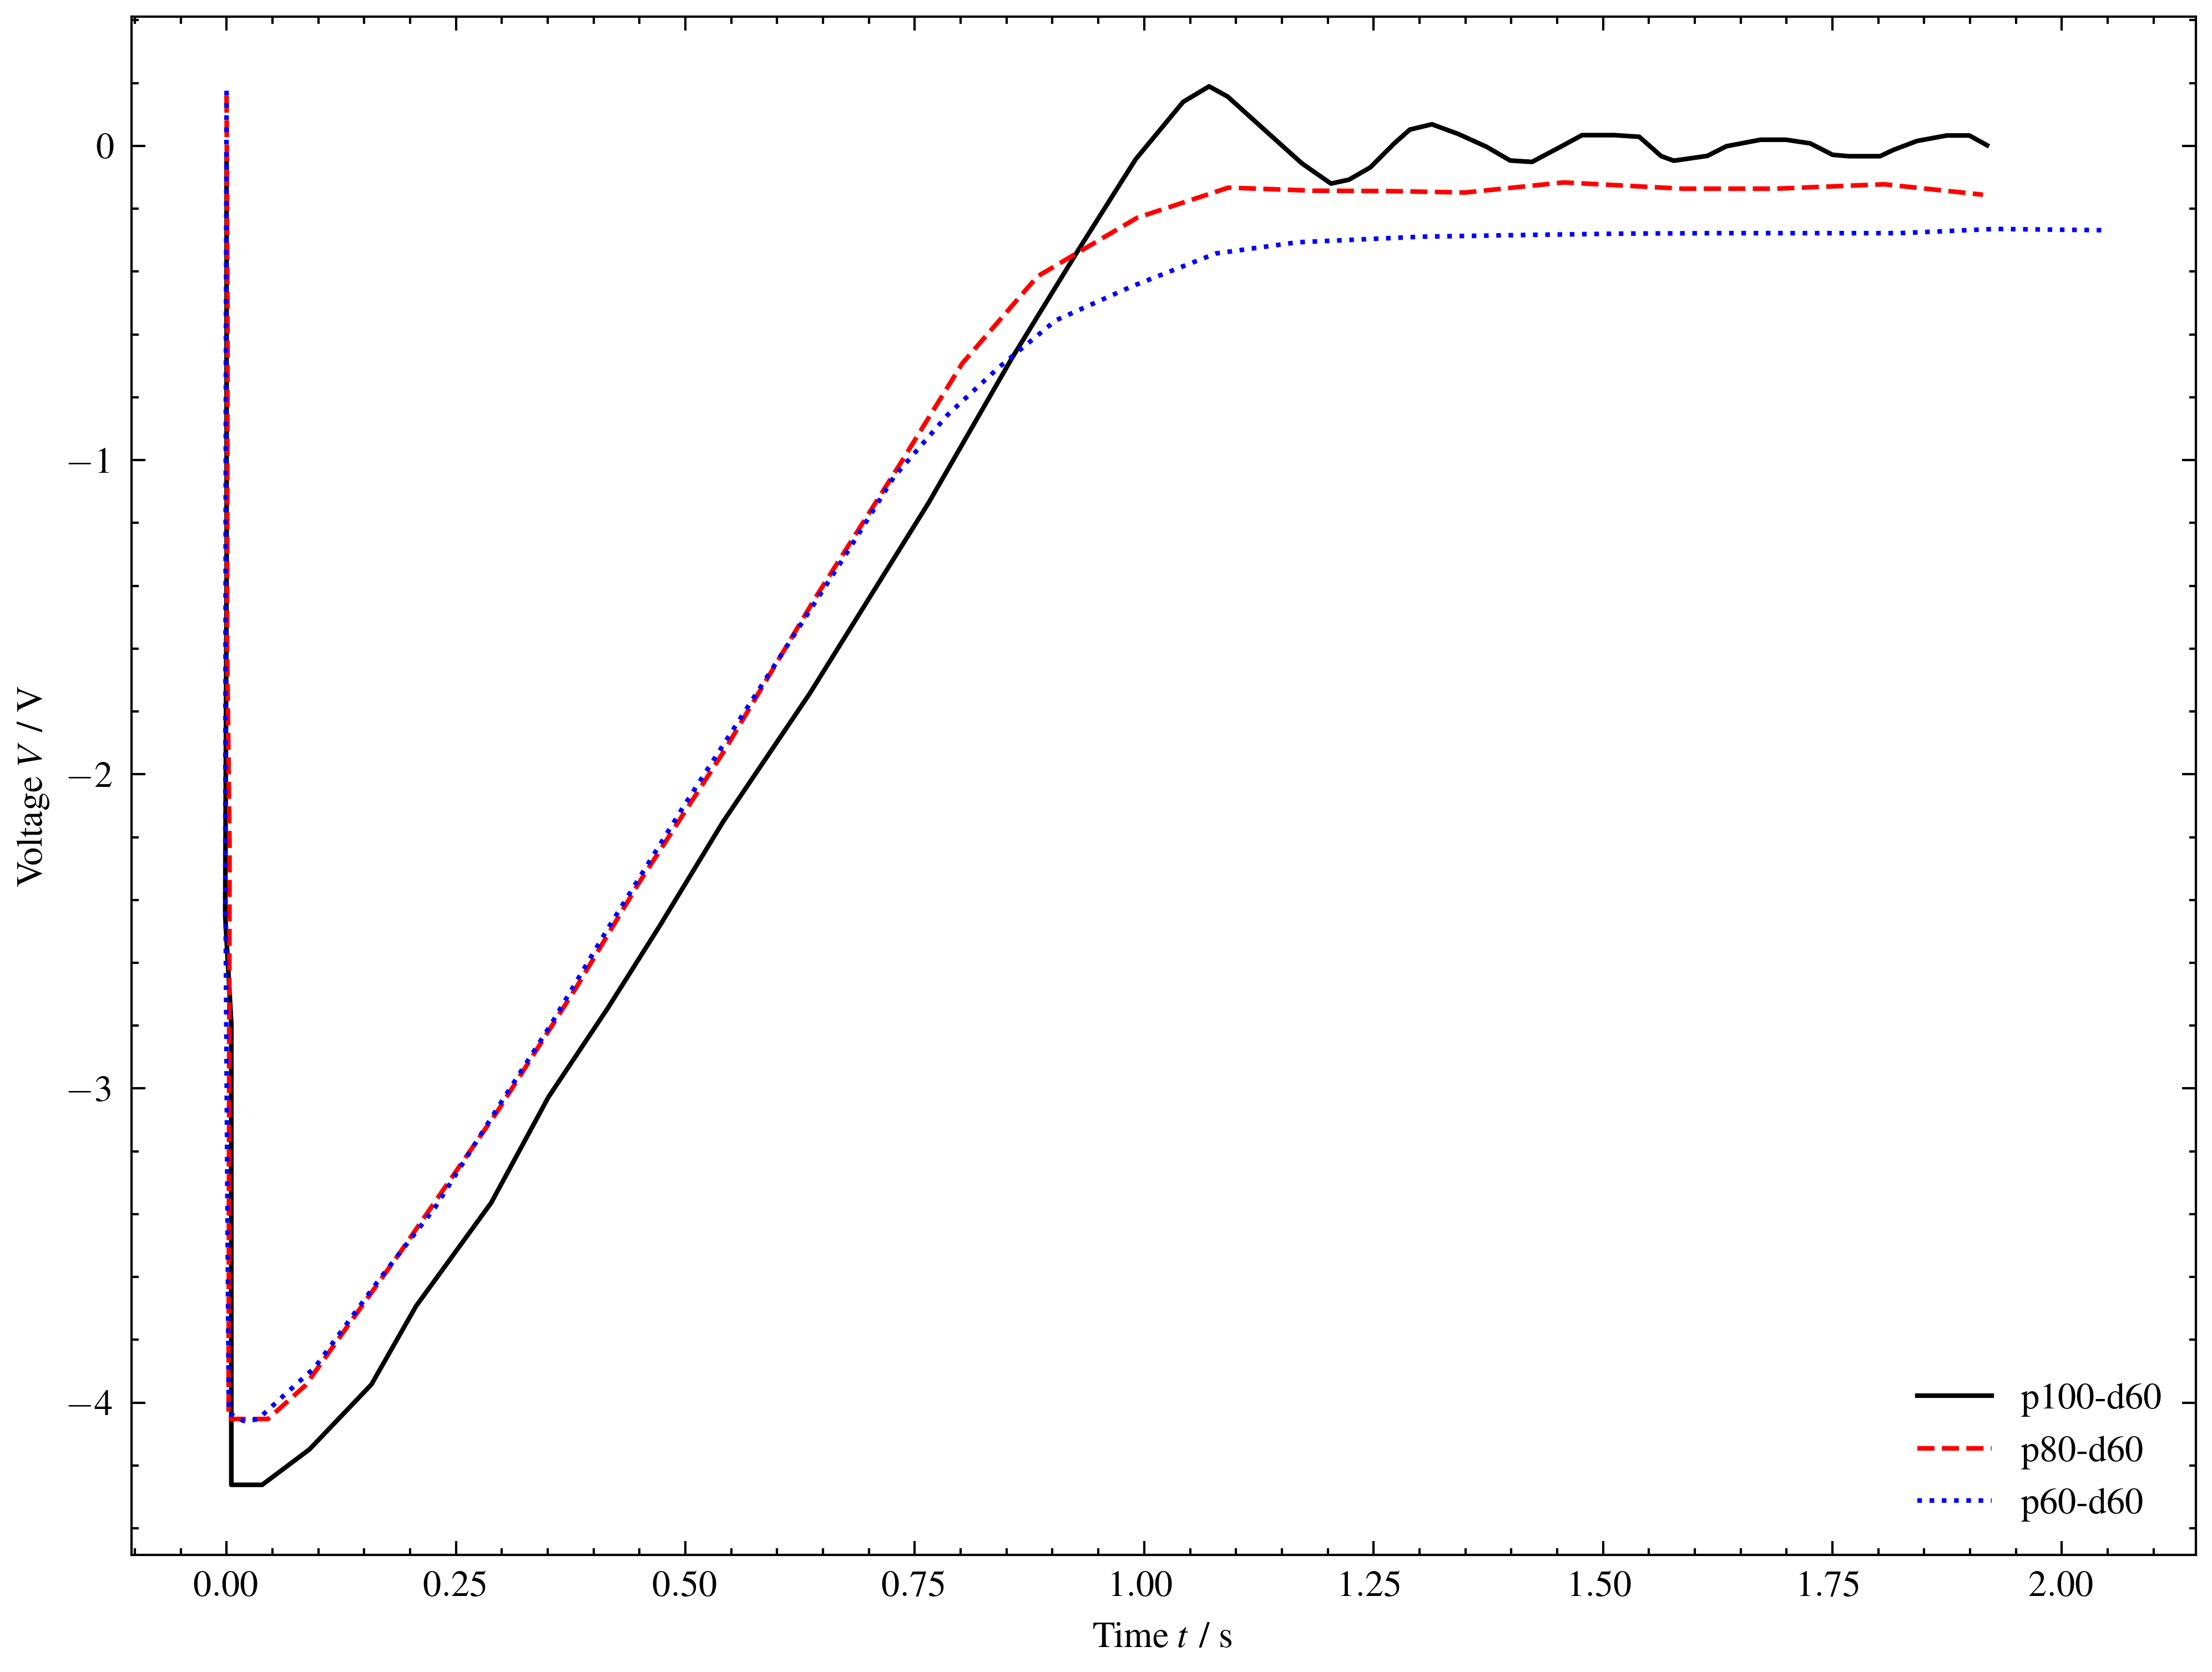
\includegraphics[width=0.8\linewidth]{src/figures/oscilloscope-grouped/d-60.png}
		\subcaption{$D = 60$}
	\end{subfigure}
	\begin{subfigure}{0.48\columnwidth}
		\centering
		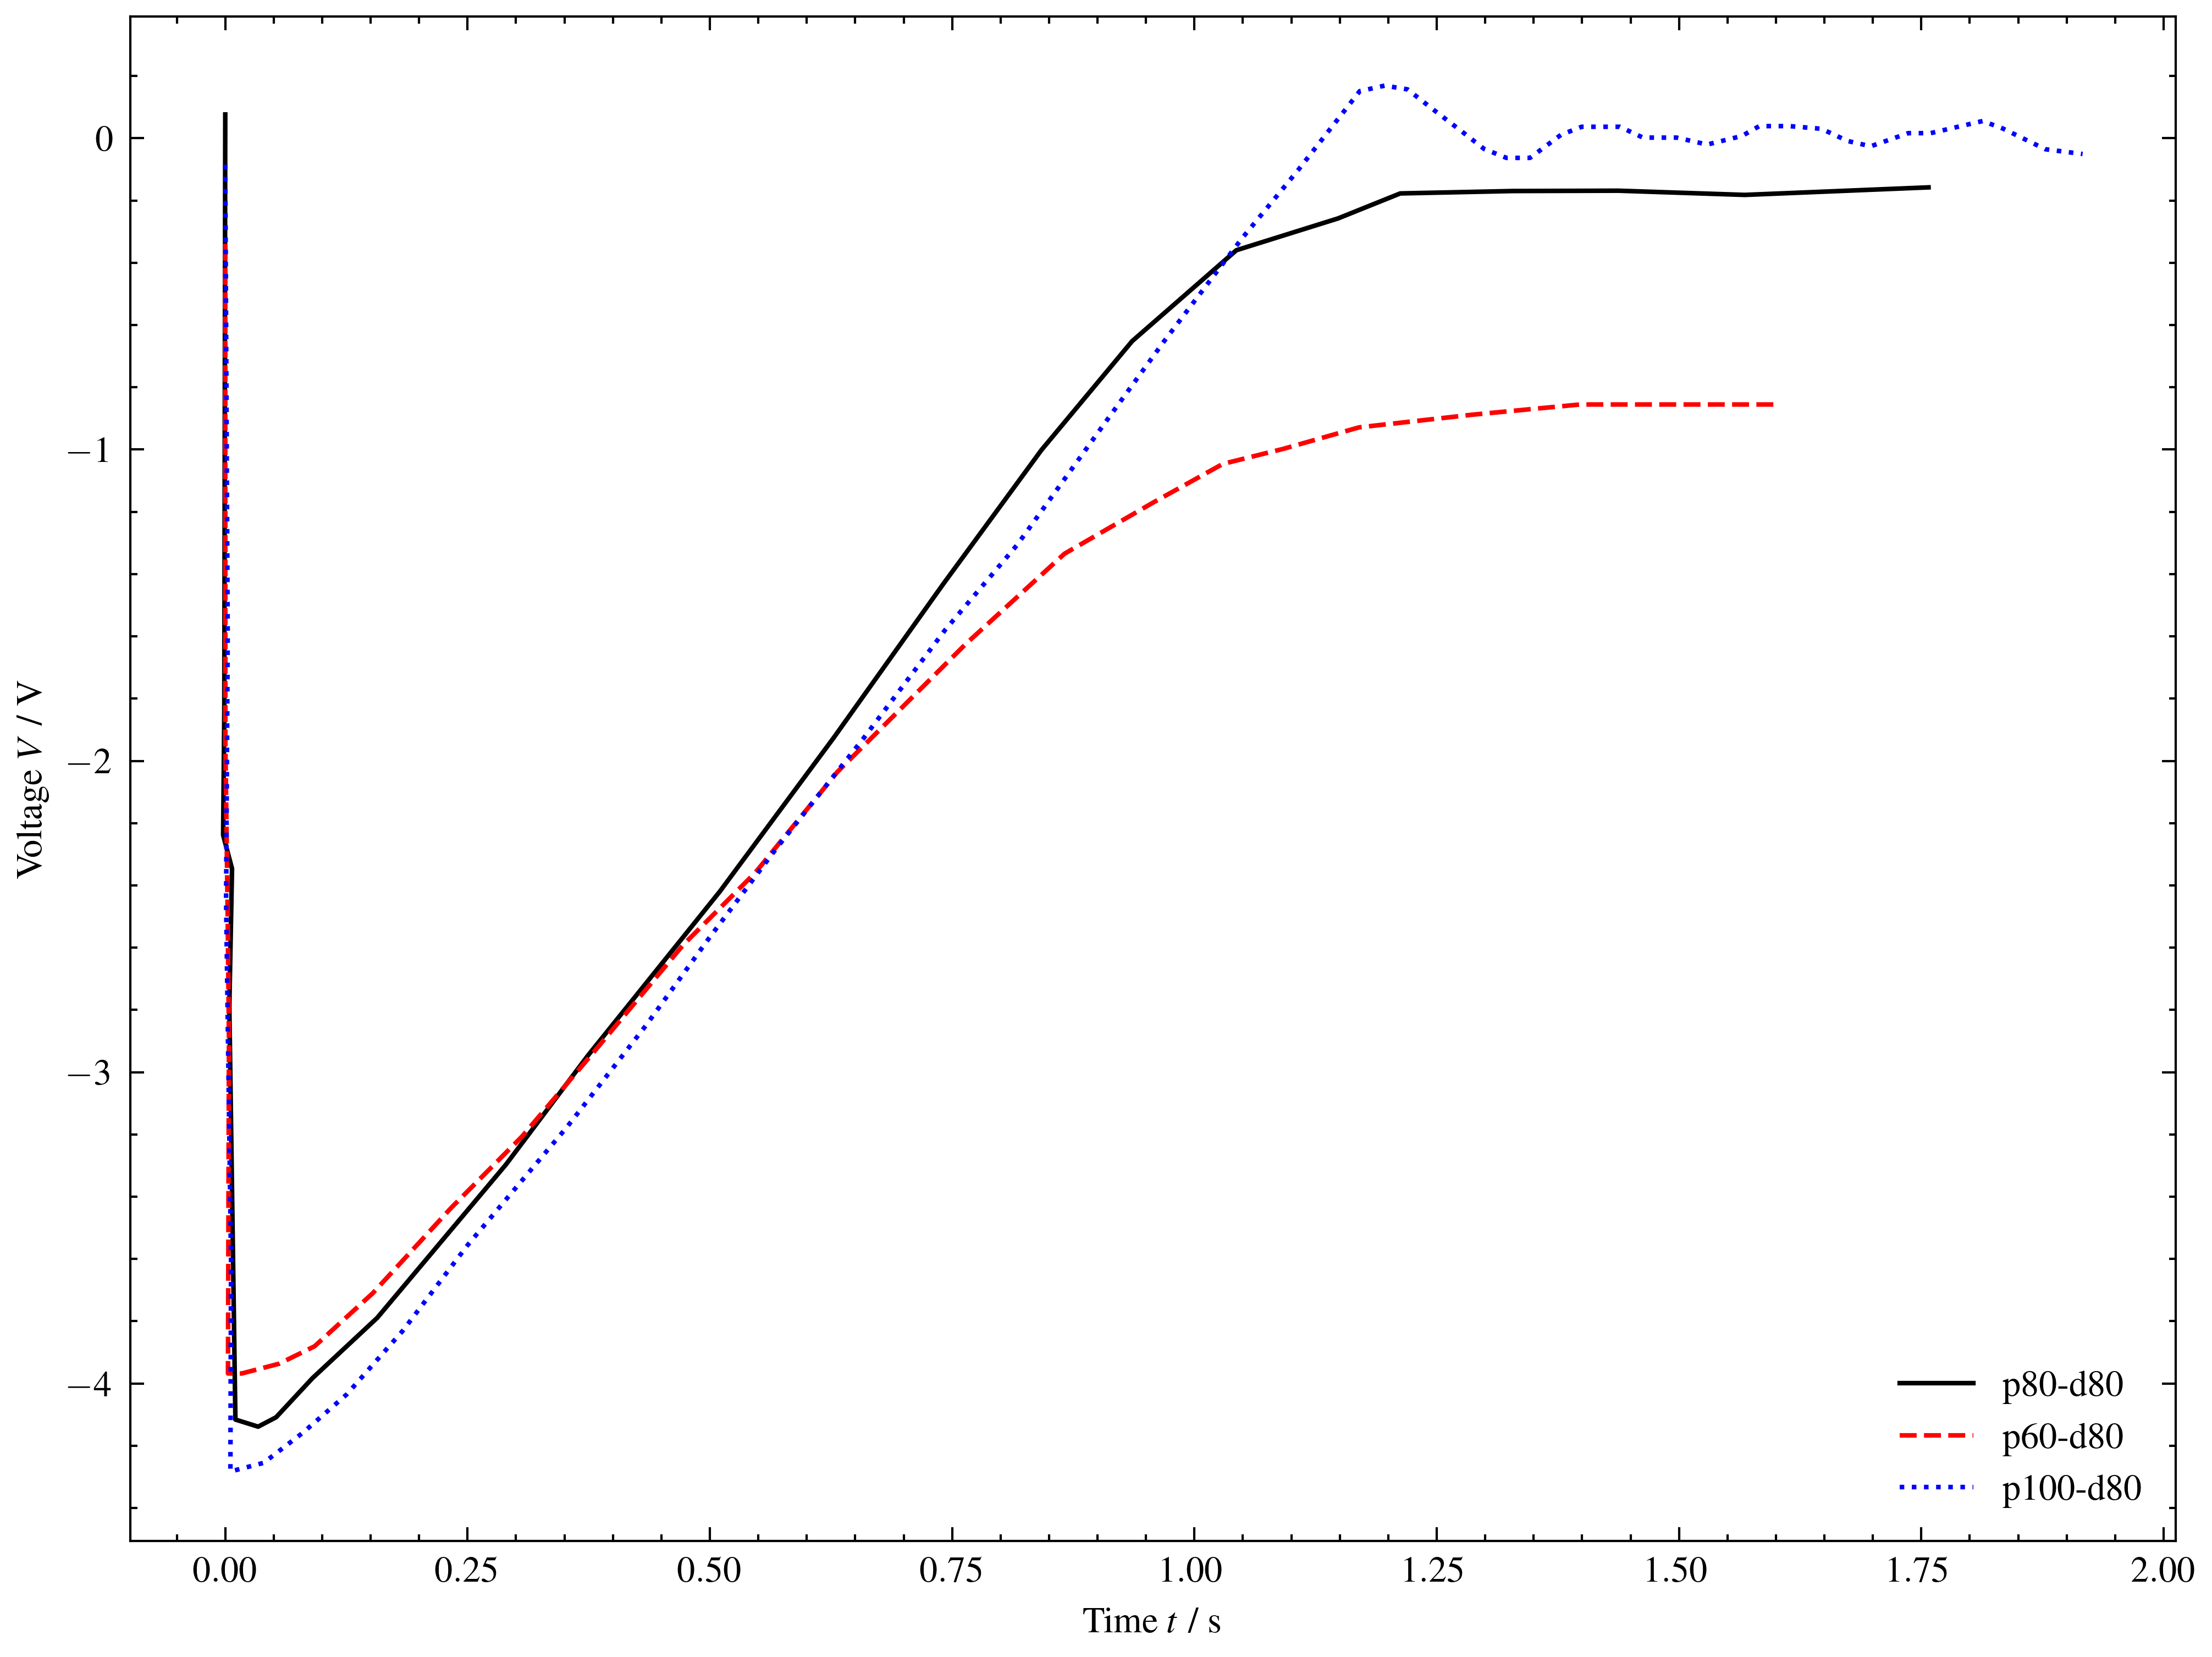
\includegraphics[width=0.8\linewidth]{src/figures/oscilloscope-grouped/d-80.png}
		\subcaption{$D = 80$}
	\end{subfigure}
	\begin{subfigure}{0.48\columnwidth}
		\centering
		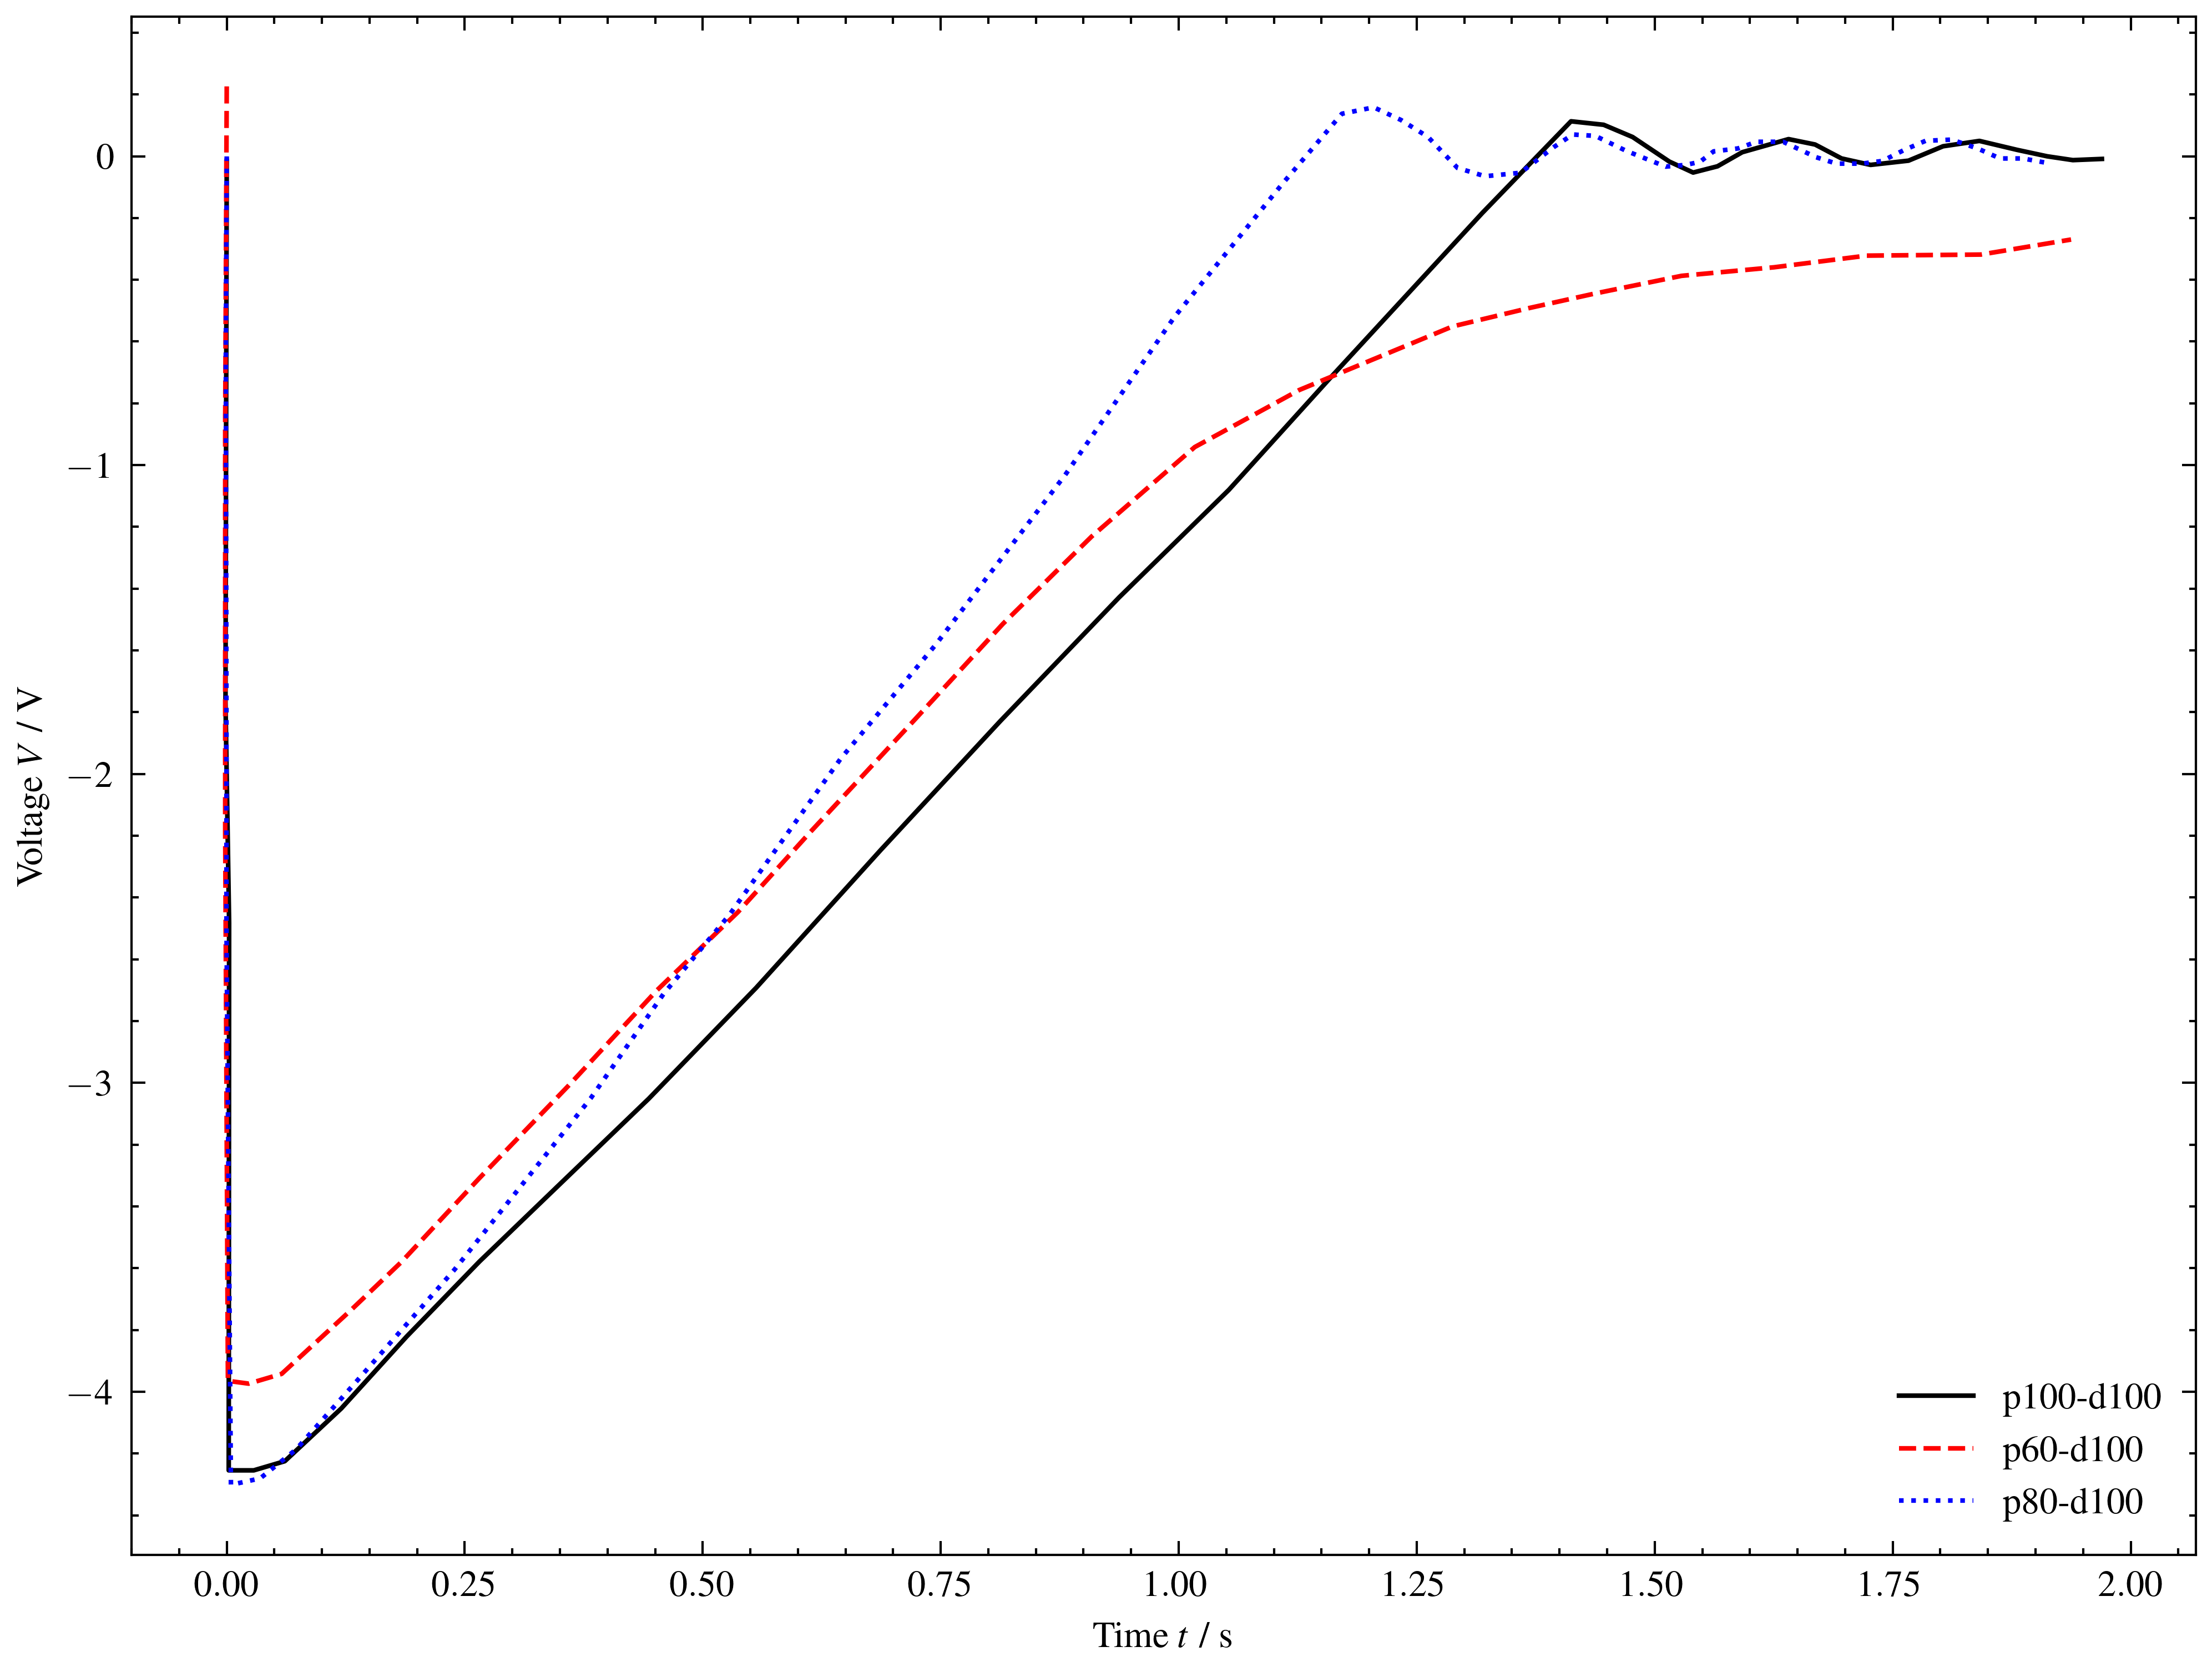
\includegraphics[width=0.8\linewidth]{src/figures/oscilloscope-grouped/d-100.png}
		\subcaption{$D = 100$}
	\end{subfigure}
	\caption{ある$D$に対する$P$を変化させたときの波形}\label{fig:oscilloscope-grouped-d}
\end{figure}

\begin{figure}
	\centering
	\begin{subfigure}{0.48\columnwidth}
		\centering
		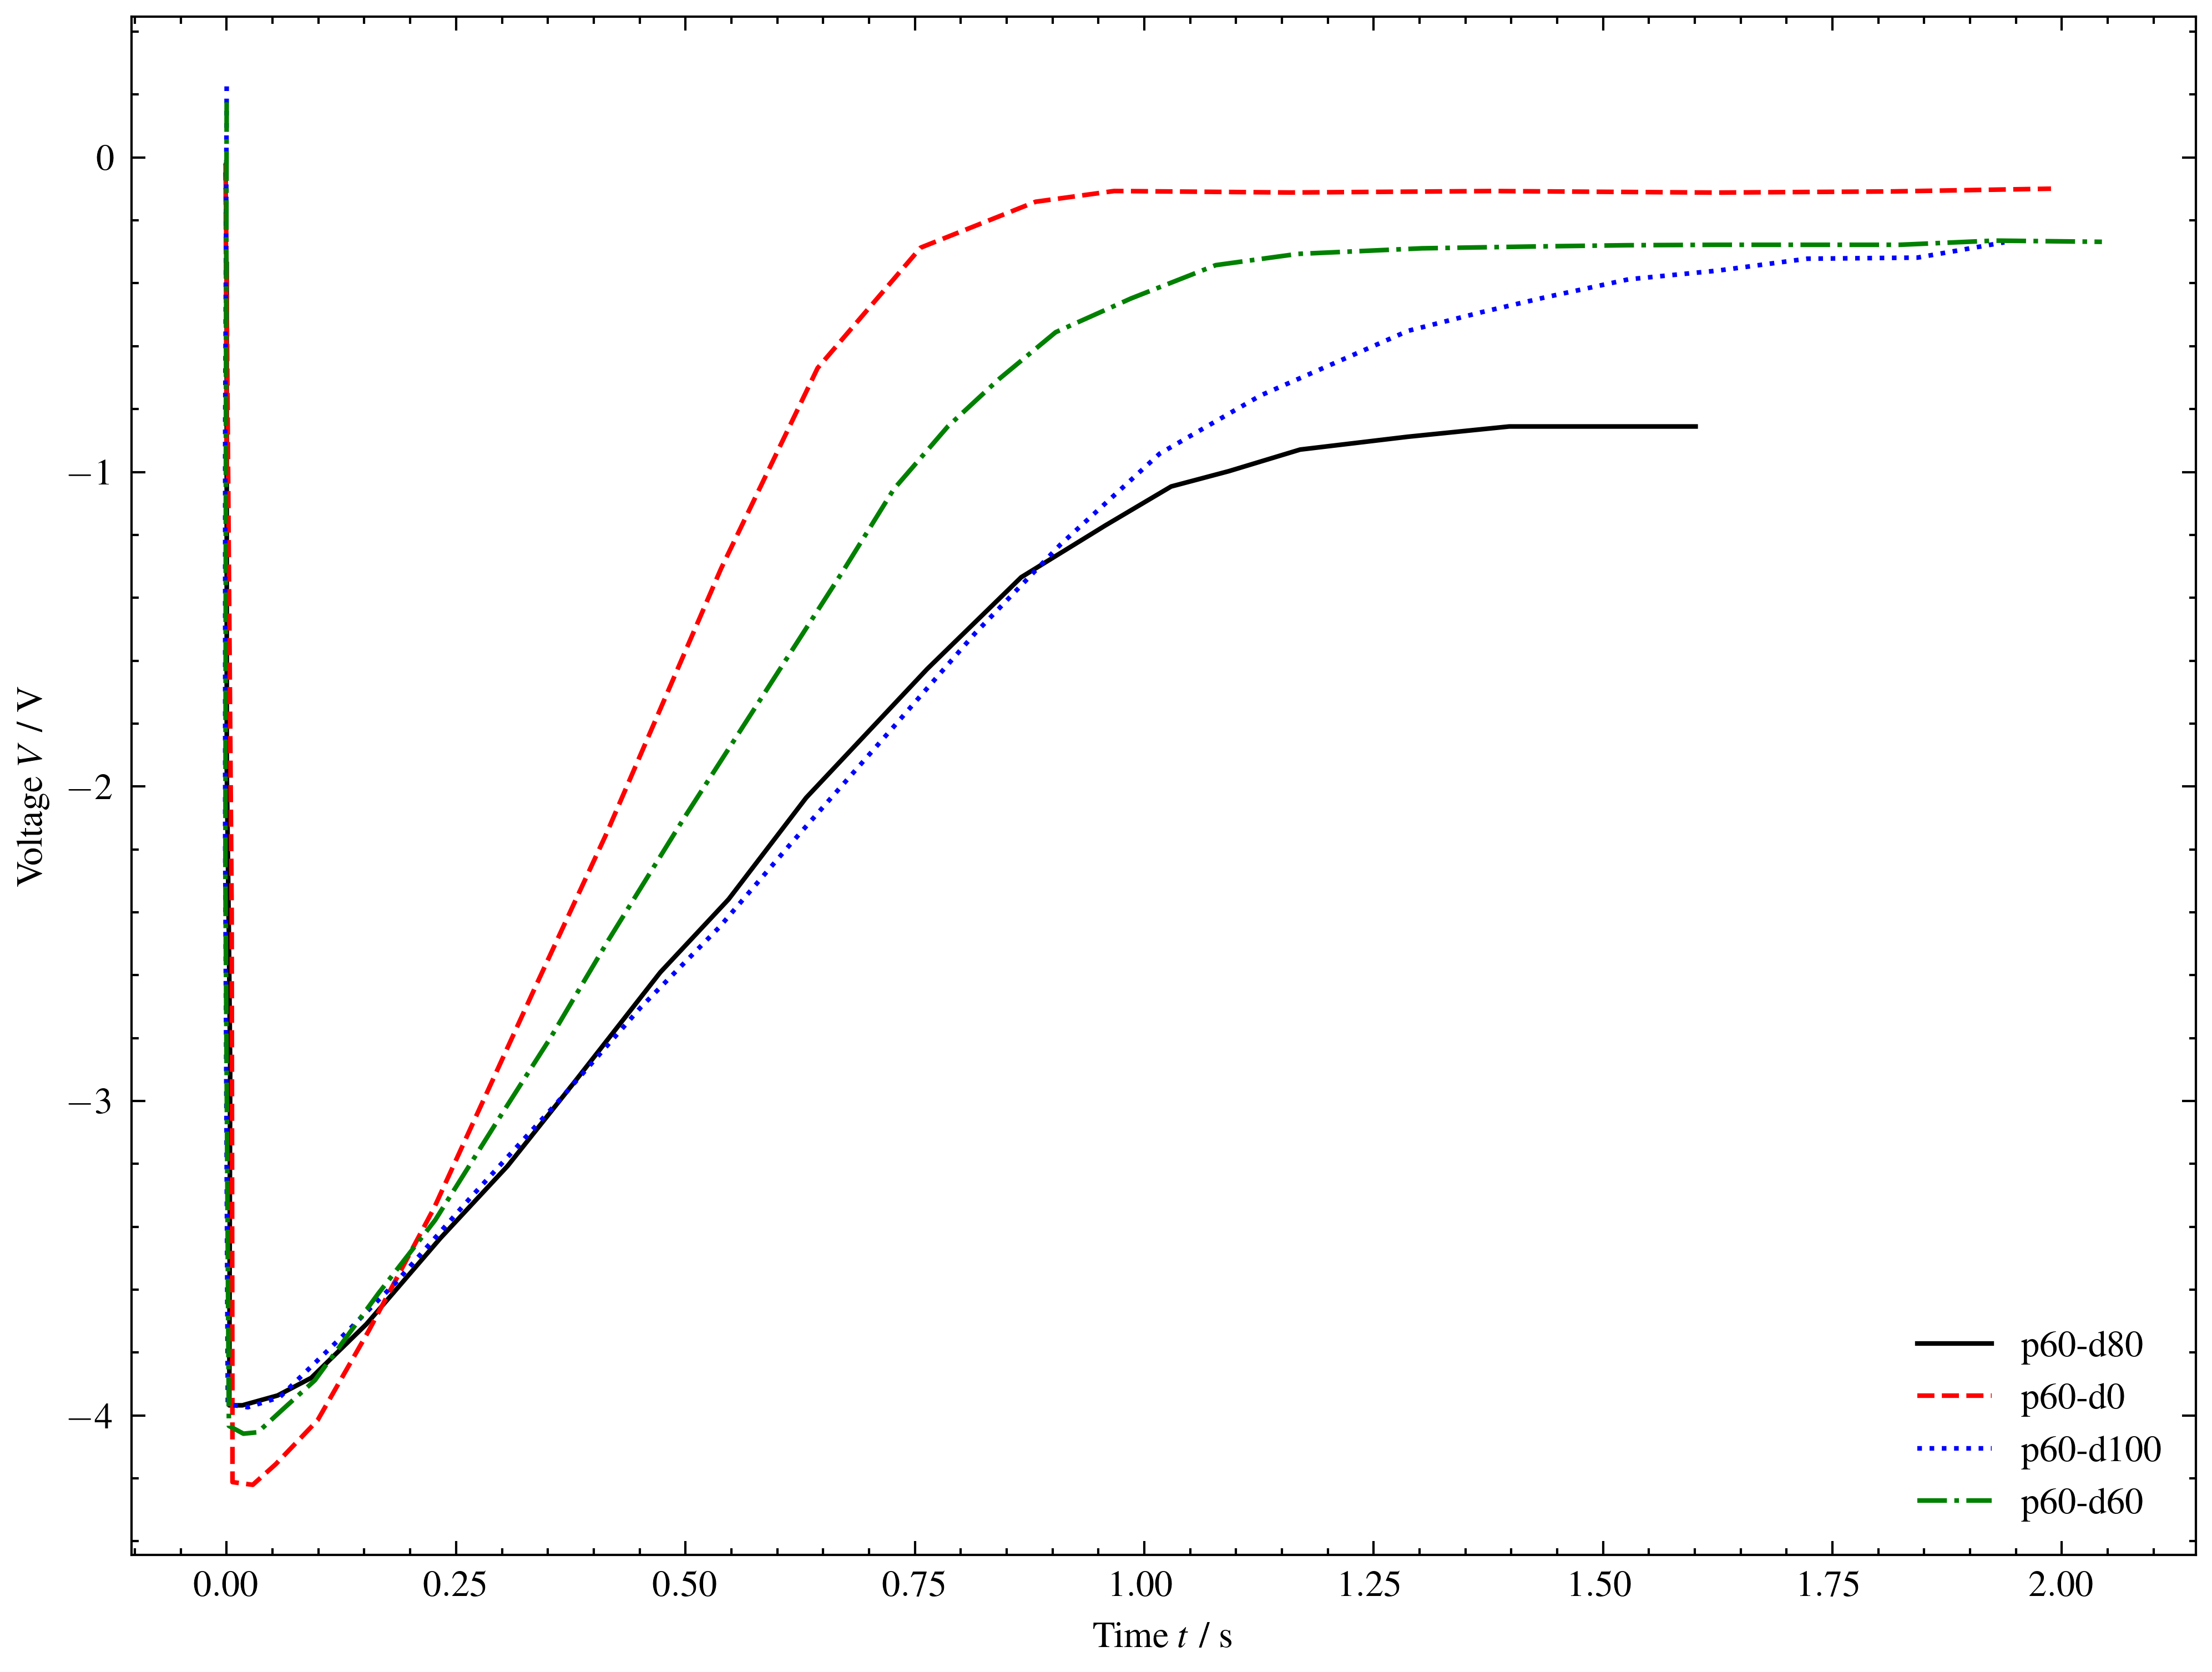
\includegraphics[width=0.8\linewidth]{src/figures/oscilloscope-grouped/p-60.png}
		\subcaption{$P = 60$}
	\end{subfigure}
	\begin{subfigure}{0.48\columnwidth}
		\centering
		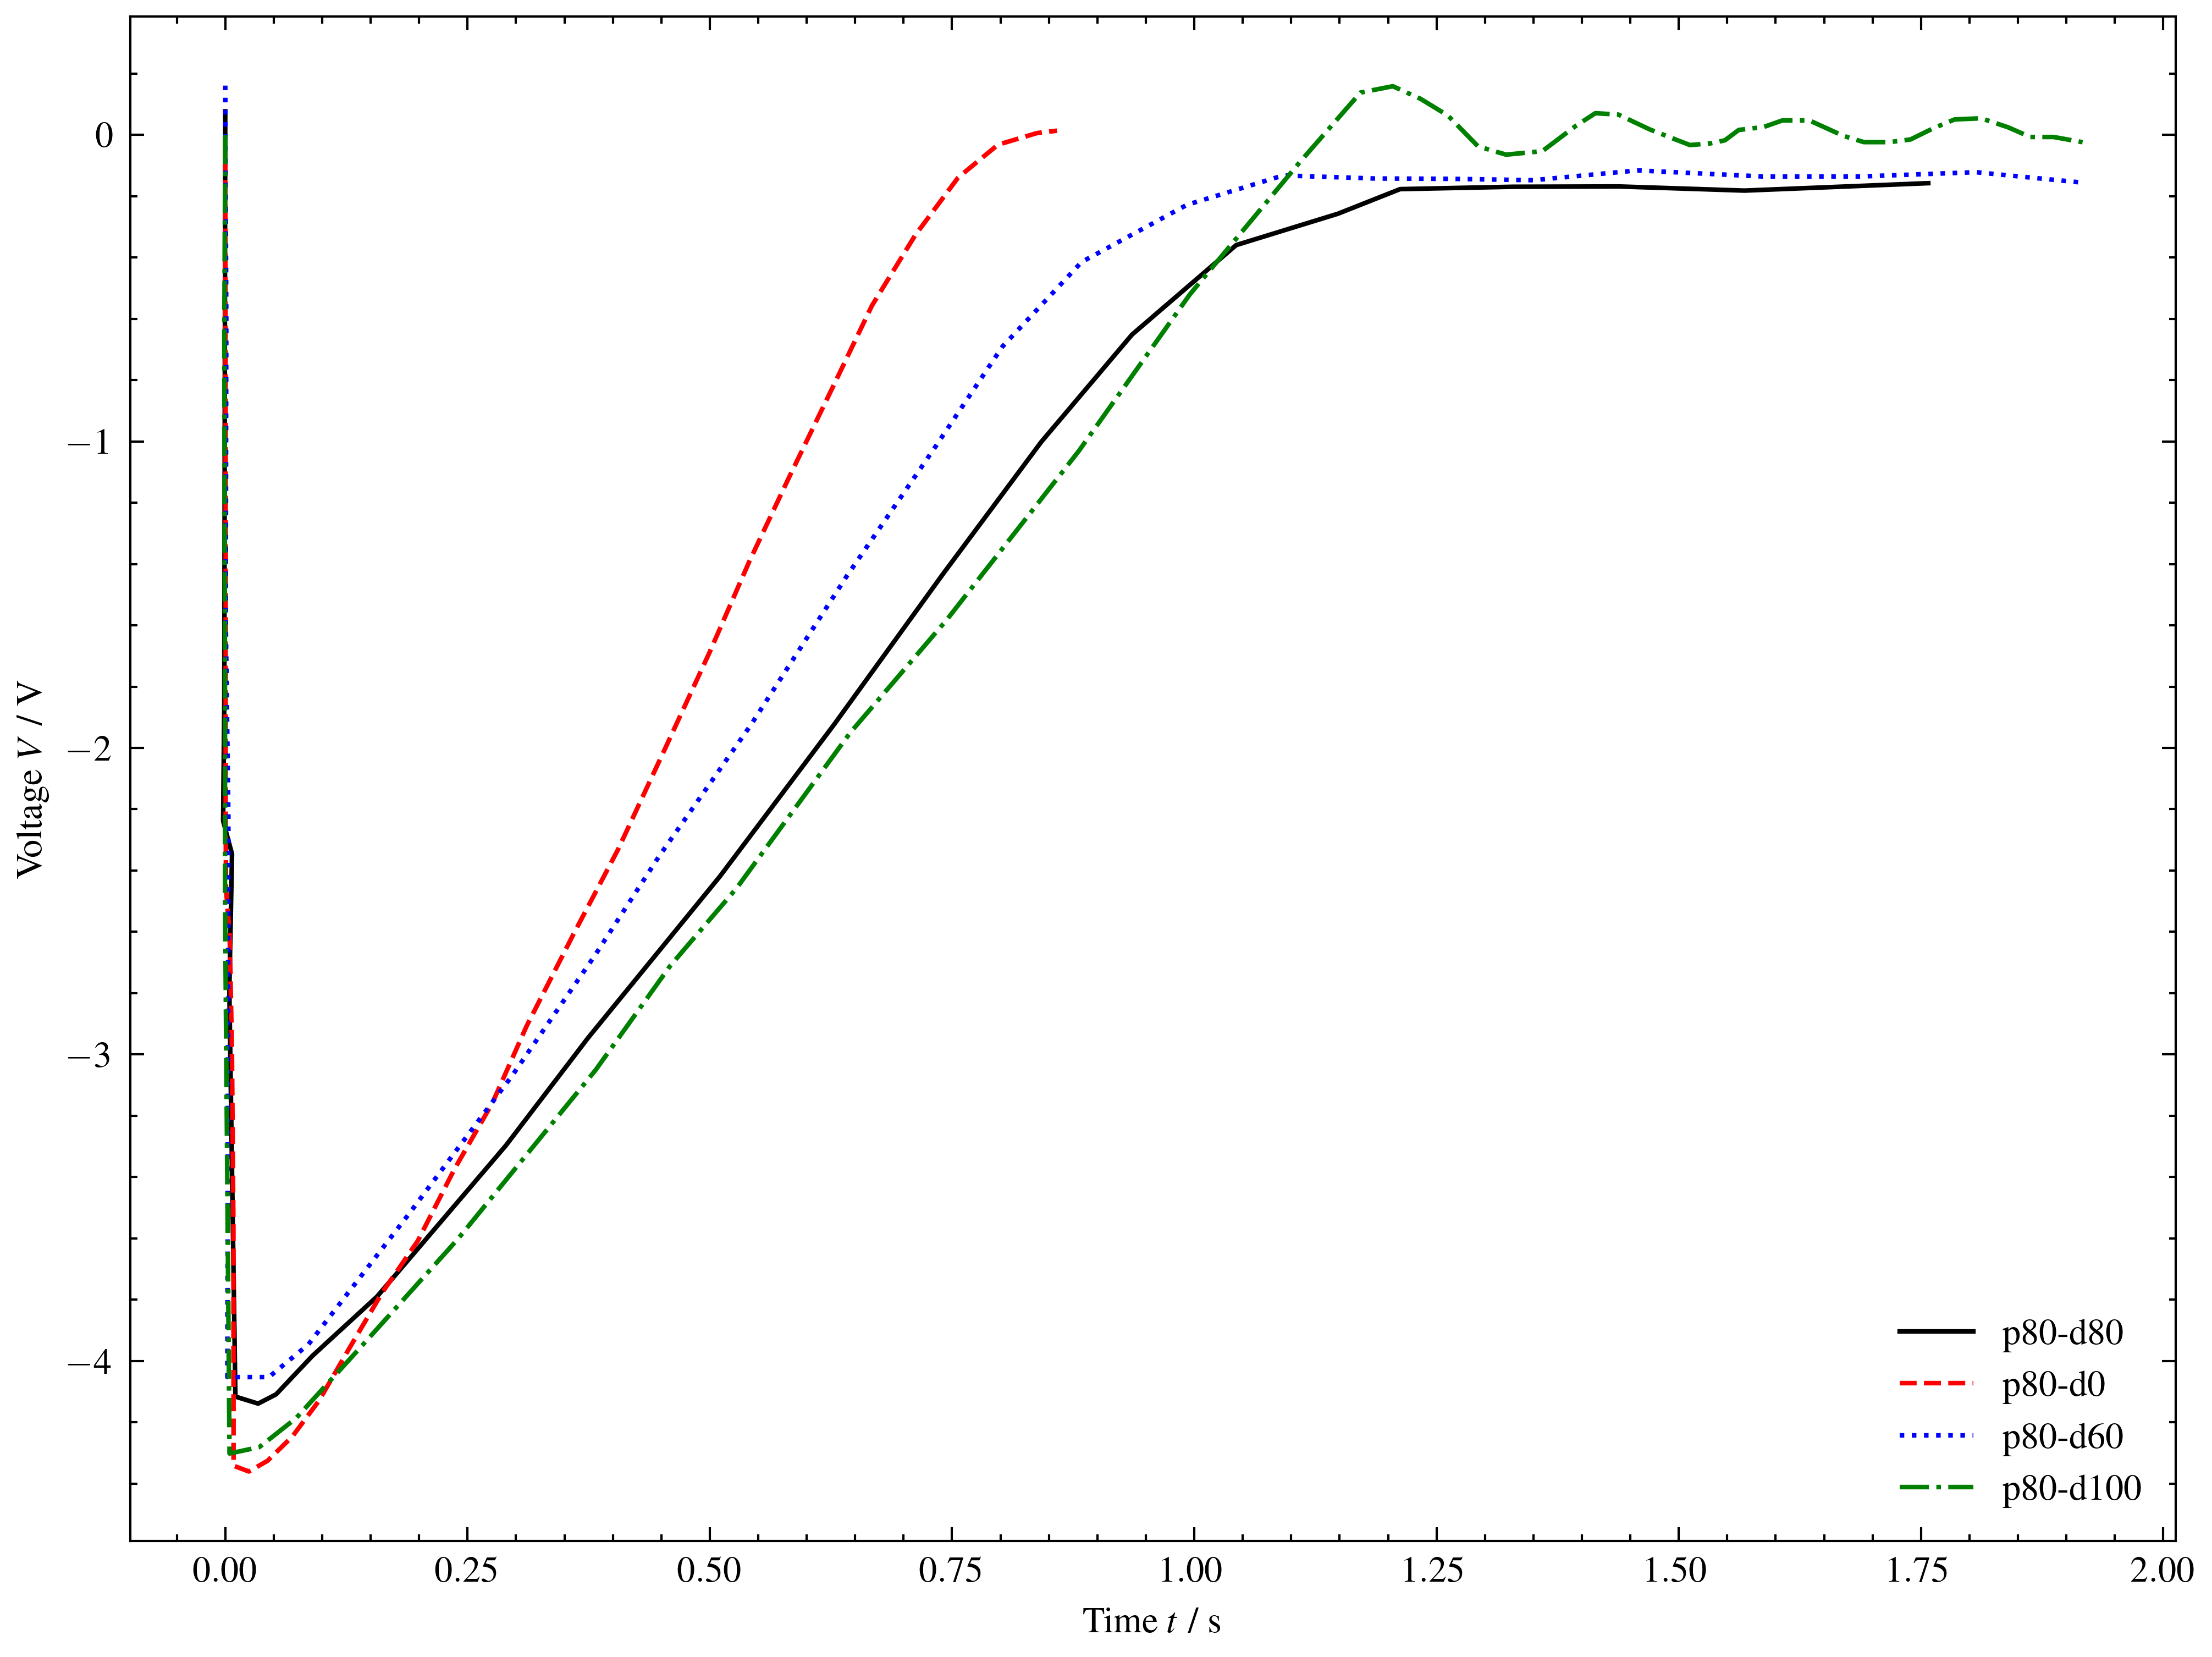
\includegraphics[width=0.8\linewidth]{src/figures/oscilloscope-grouped/p-80.png}
		\subcaption{$P = 80$}
	\end{subfigure}
	\begin{subfigure}{0.48\columnwidth}
		\centering
		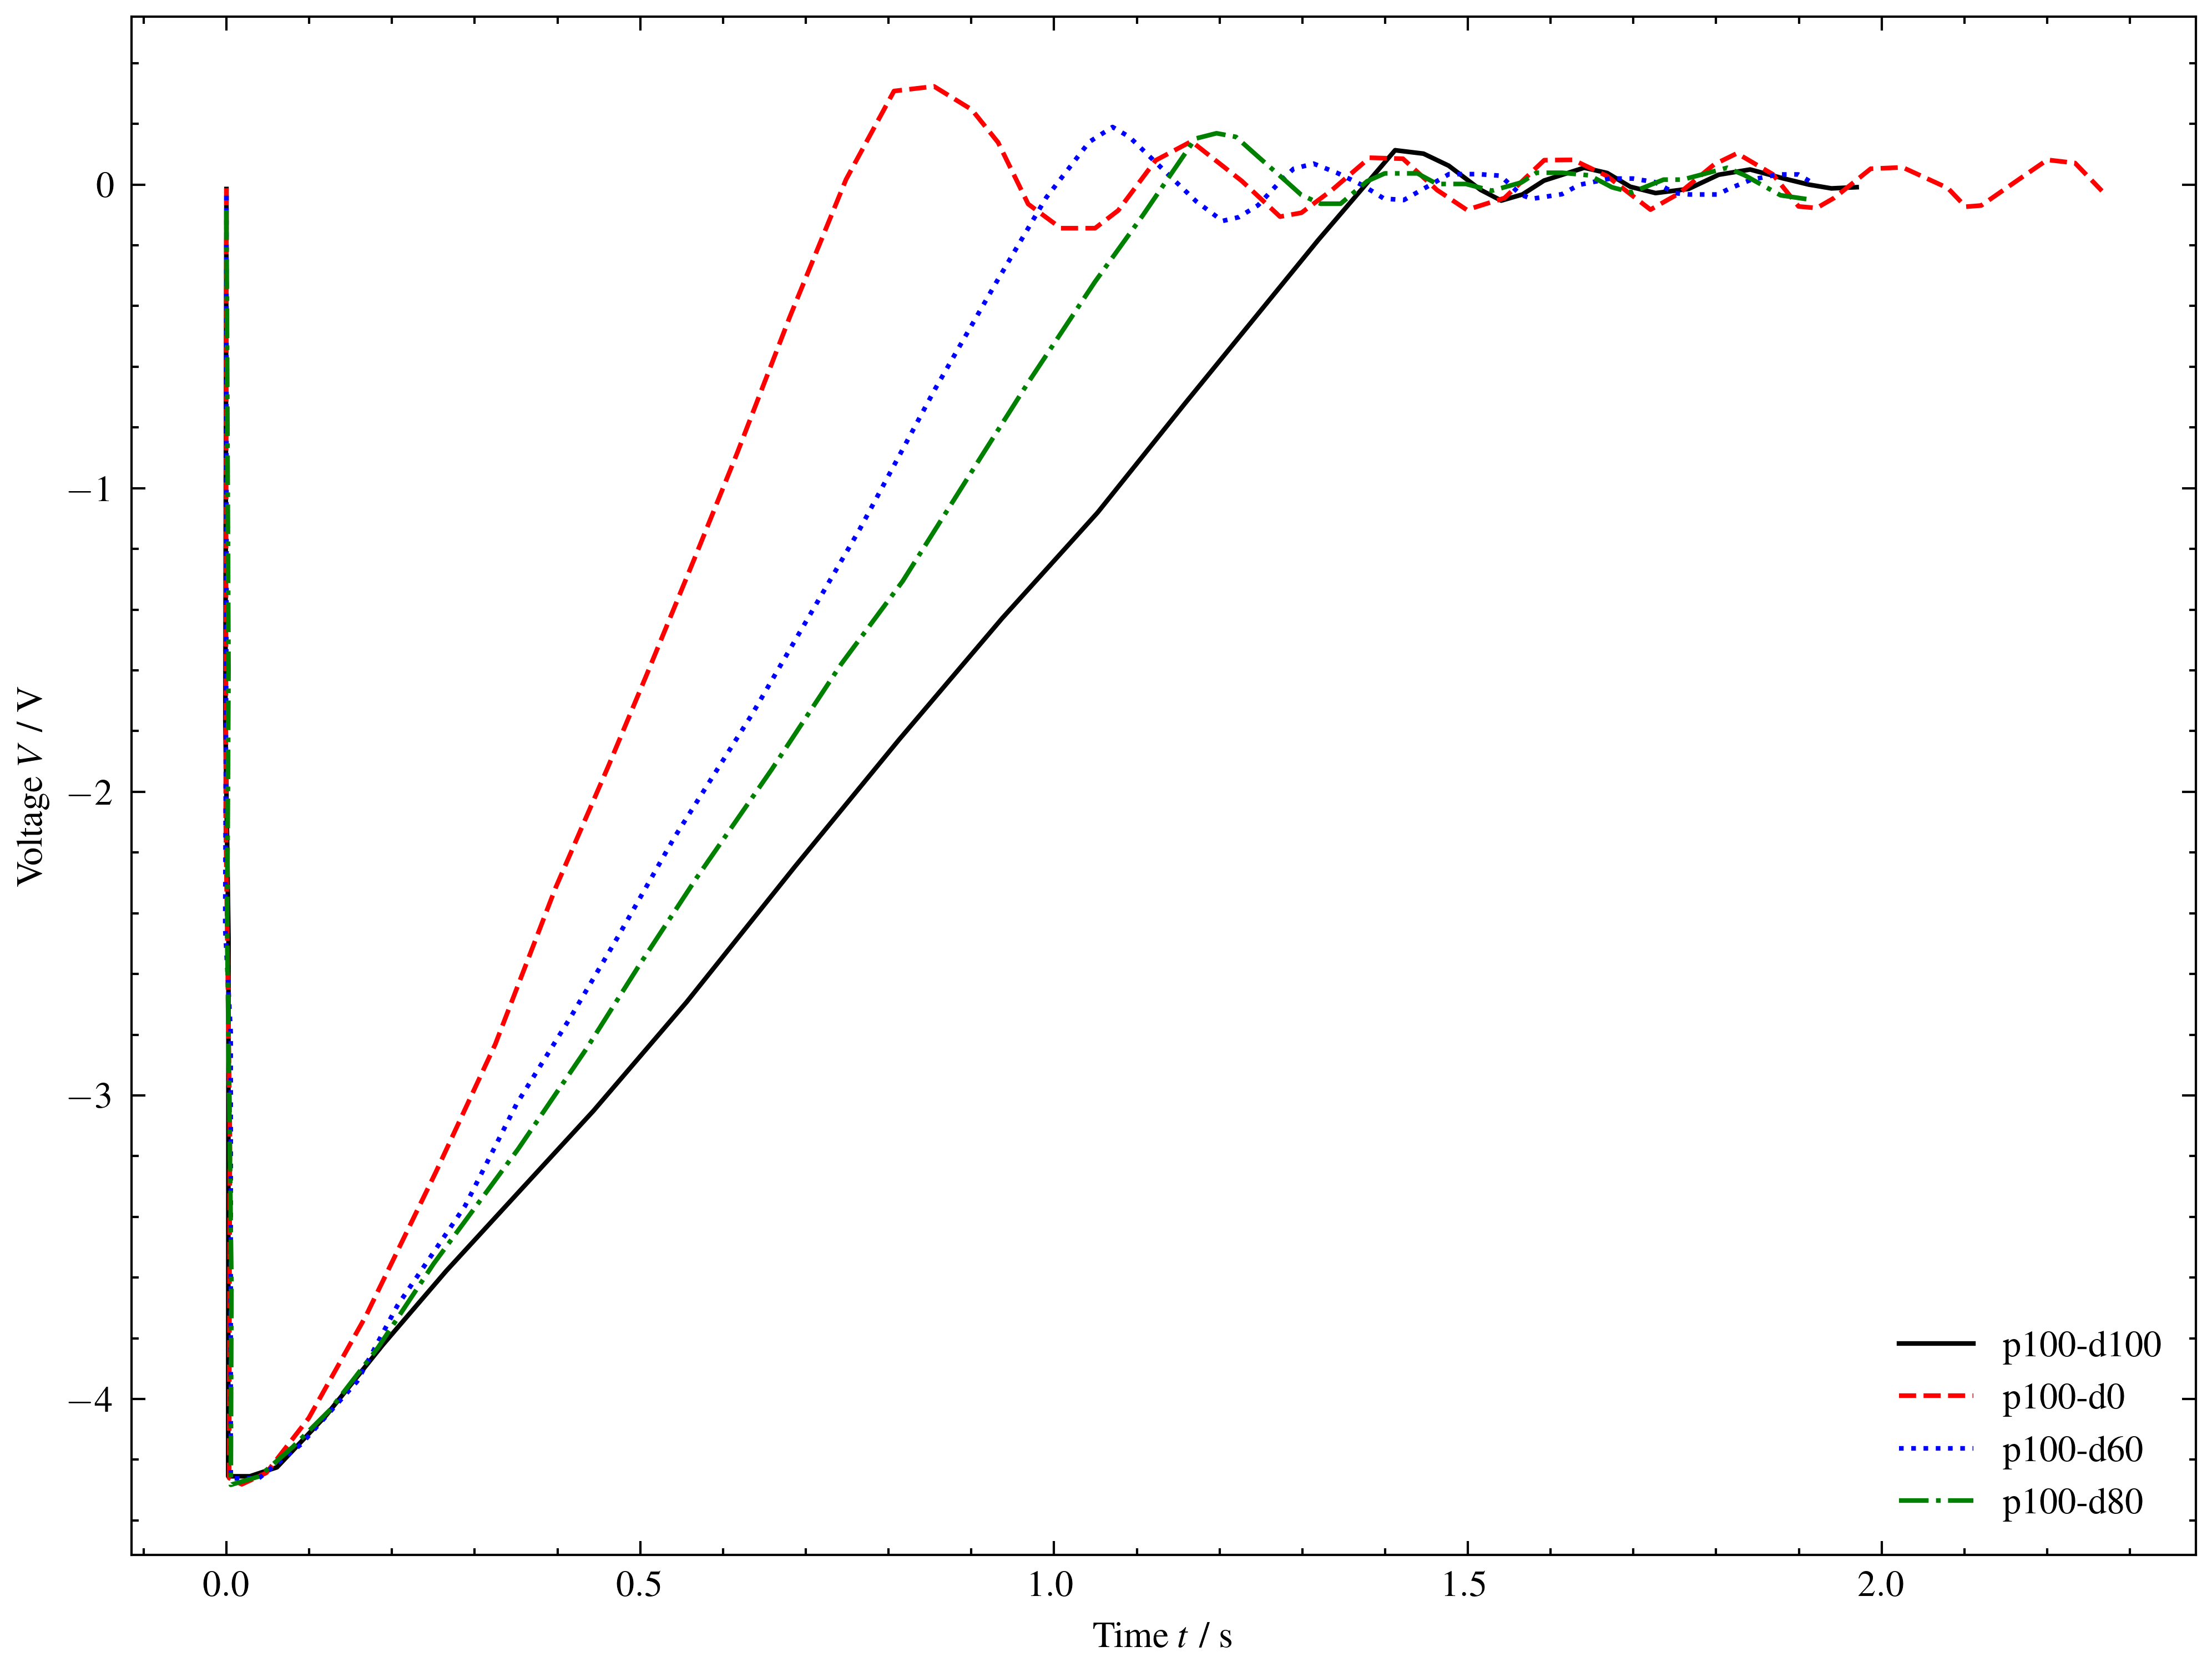
\includegraphics[width=0.8\linewidth]{src/figures/oscilloscope-grouped/p-100.png}
		\subcaption{$P = 100$}
	\end{subfigure}
	\caption{ある$P$に対する$D$を変化させたときの波形}\label{fig:oscilloscope-grouped-p}
\end{figure}
